\documentclass{warpdoc}
\newlength\lengthfigure                  % declare a figure width unit
\setlength\lengthfigure{0.158\textwidth} % make the figure width unit scale with the textwidth
\usepackage{psfrag}         % use it to substitute a string in a eps figure
\usepackage{subfigure}
\usepackage{rotating}
\usepackage{pstricks}
\usepackage[innercaption]{sidecap} % the cute space-saving side captions
\usepackage{scalefnt}
\usepackage{amsbsy}
\usepackage{amsmath}
\usepackage{bm}
\numberwithin{equation}{section}

%%%%%%%%%%%%%=--NEW COMMANDS BEGINS--=%%%%%%%%%%%%%%%%%%%%%%%%%%%%%%%%%%
\newcommand{\alb}{\vspace{0.2cm}\\} % array line break
\newcommand{\rhos}{\rho}
\newcommand{\Cv}{{c_{v}}}
\newcommand{\Cp}{{c_{p}}}
\newcommand{\Sct}{{{\rm Sc}_{\rm t}}}
\newcommand{\Prt}{{{\rm Pr}_{\rm t}}}
\newcommand{\nd}{{{n}_{\rm d}}}
\newcommand{\ns}{{{n}_{\rm s}}}
\newcommand{\nn}{{{n}_{\rm n}}}
\newcommand{\ndm}{{\bar{n}_{\rm d}}}
\newcommand{\nsm}{{\bar{n}_{\rm s}}}
\newcommand{\turb}{_{\rm t}}
\newcommand{\mut}{{\mu\turb}}
\newcommand{\mfa}{\scriptscriptstyle}
\newcommand{\mfb}{\scriptstyle}
\newcommand{\mfc}{\textstyle}
\newcommand{\mfd}{\displaystyle}
\newcommand{\hlinex}{\vspace{-0.34cm}~~\\ \hline \vspace{-0.31cm}~~\\}
\newcommand{\hlinextop}{\vspace{-0.46cm}~~\\ \hline \hline \vspace{-0.32cm}~~\\}
\newcommand{\hlinexbot}{\vspace{-0.37cm}~~\\ \hline \hline \vspace{-0.50cm}~~\\}
\newcommand{\tablespacing}{\vspace{-0.4cm}}
\newcommand{\fontxfig}{\footnotesize\scalefont{0.918}}
\newcommand{\fontgnu}{\footnotesize\scalefont{0.896}}
\newcommand{\ordi}{{\rm d}}
\newcommand{\Acs}{A_{\rm cs}}
\newcommand{\mdot}{\dot{m}}
\newcommand{\bigfrac}{\mfd\frac}
\newcommand\frameeqn[1]{\fbox{$#1$}}
\renewcommand{\fontsizetable}{\footnotesize\scalefont{1.0}}
\renewcommand{\fontsizefigure}{\footnotesize}
\renewcommand{\vec}[1]{\bm{#1}}
\setcounter{tocdepth}{3}
\let\citen\cite

%%%%%%%%%%%%%=--NEW COMMANDS BEGINS--=%%%%%%%%%%%%%%%%%%%%%%%%%%%%%%%%%%

\setcounter{tocdepth}{3}

%%%%%%%%%%%%%=--NEW COMMANDS ENDS--=%%%%%%%%%%%%%%%%%%%%%%%%%%%%%%%%%%%%



\author{
  Bernard Parent
}

\email{
  bernparent@gmail.com
}

\department{
  Institute for Aerospace Studies	
}

\institution{
  University of Toronto
}

\title{
  Performance Parameters
}

\date{
  June 2001
}

%\setlength\nomenclaturelabelwidth{0.13\hsize}  % optional, default is 0.03\hsize
%\setlength\nomenclaturecolumnsep{0.09\hsize}  % optional, default is 0.06\hsize

\nomenclature{

  \begin{nomenclaturelist}{Roman symbols}
   \item[$a$] speed of sound
  \end{nomenclaturelist}
}


\abstract{
abstract
}

\begin{document}
  \pagestyle{headings}
  \pagenumbering{arabic}
  \setcounter{page}{1}
%%  \maketitle
  \makewarpdoctitle
%  \makeabstract
  \tableofcontents
%  \makenomenclature
%%  \listoftables
%%  \listoffigures



\section{Stagnation Pressure}


The stagnation pressure is defined as the pressure obtained from the integration
of the governing equations (in differential Euler form)
till the velocity vanishes along a streamline. Defining $s$ as
the coordinate following a streamline, we can write the continuity,
momentum and energy equations at steady-state as:
%
\begin{displaymath}
 \begin{array}{c@{~~~~~}l}
  \bigfrac{\ordi }{\ordi s}\rho  u \Acs =0 & {\rm continuity}\alb
  \bigfrac{\ordi }{\ordi s}\rho u^2 \Acs+\bigfrac{\ordi }{\ordi s} P \Acs
     =-P \bigfrac{\ordi \Acs}{\ordi s} & {\rm momentum}\alb
  \bigfrac{\ordi }{\ordi s}\rho  u \Acs h_{\rm t} =0 & {\rm energy}\alb
 \end{array}
\end{displaymath}
%
with $h_{\rm t}$ the total enthalpy ($h_{\rm t}\equiv h + u^2/2$). Subtracting the continuity
from the momentum and energy gives us the primitive form,
%
\begin{displaymath}
 \begin{array}{c@{~~~~~}l}
  \rho u \bigfrac{\ordi u}{\ordi s} =-\bigfrac{\ordi P}{\ordi s} & {\rm momentum}\alb
  \bigfrac{\ordi h_{\rm t}}{\ordi s} =0 & {\rm energy}
 \end{array}
\end{displaymath}
%
which we seek to integrate from state 1 to state 2
(subsequently referred to by the subscripts 1 and 2 respectively).
The equations are written
in quasi-1D formulation to reflect a possible change of cross-flow
area along the streamline. Interestingly, the primitive form of the momentum
equation and of the energy equation is unchanged.


\subsection{Incompressible Flow}

In the case of
an \emph{incompressible flow}, the energy equation is not needed to integrate the
momentum, as $\rho$ is constant and there is no link between $P$ and $T$. Hence,
the integration of the momentum equation can be written as,
%
\begin{equation}
  \rho \int_{u_1}^{u_2} u \ordi u = - \int_{P_1}^{P_2} \ordi P
\end{equation}
%
which yields
%
\begin{equation}
  \frameeqn{
    \mfd P_2 = P_1 + \frac{\rho u_1^2}{2}
  }
\end{equation}
%
which is the Bernoulli equation.



\subsection{Perfect Gas}

For a thermally and calorically perfect gas the energy equation
has to be taken into account as the density is a function of the
pressure and temperature, the latter needing the energy equation
to be determined, which is readily integrated to:
%
\begin{equation}
  \int_{{(h_{\rm t})}_1}^{h_{\rm t}} \ordi h_{\rm t} =0
\end{equation}
%
or
%
\begin{equation}
  h + \bigfrac{u^2}{2} = h_1 + \bigfrac{u_1^2}{2}
\end{equation}
%
From the ideal gas equation of state, we can say, (using the definition
$h\equiv \Cp T$)
%
\begin{equation}
  \rho=\bigfrac{P}{RT}=\bigfrac{\Cp P}{Rh}
      =\bigfrac{\Cp P}{R(h_1+u_1^2/2-u^2/2)}
\end{equation}
%
which we substitute back in the momentum equation $ \rho u \ordi u =-\ordi P$
to get:
%
\begin{equation}
  2 \int_{u_1}^{u_2} \bigfrac{u}{(2 h_1+u_1^2-u^2)}  \ordi u
  =-\int_{P_1}^{P_2} \frac{R}{\Cp P}\ordi P
\end{equation}
%
After integration, this becomes:
%
\begin{equation}
  -\ln (2 h_1+u_1^2-u_2^2)
  +\ln (2 h_1+u_1^2-u_1^2)
  =- \frac{R}{\Cp}\ln (P_2/P_1)
\end{equation}
%
Using $\gamma \equiv \Cp/\Cv$ and $R=\Cp-\Cv$, and rearranging:
%
\begin{equation}
   \frac{\gamma}{\gamma-1} \ln ((h_1+u_1^2/2-u_2^2/2)/h_1)
  =\ln (P_2/P_1)
\end{equation}
%
which is equivalent to (since at stagnation $u_2=0$):
%
\begin{equation}
P_2=P_1 \left[  1+\frac{u_1^2}{2 h_1} \right]^\frac{\gamma}{\gamma-1}
\end{equation}
%
The enthalpy can be shown to be equal to $h=(\gamma R T)/(\gamma-1)$,
which transforms the latter into:
%
\begin{equation}
P_2=P_1 \left[  1+\frac{\gamma-1}{2} \frac{u_1^2}{\gamma R T_1} \right]^\frac{\gamma}{\gamma-1}
\end{equation}
%
or,
%
\begin{equation}
  \frameeqn{
    \mfd P_2=P_1 \left[  1+\frac{\gamma-1}{2} {\rm M}_1^2 \right]^\frac{\gamma}{\gamma-1}
  }
\end{equation}
%
It is noted that in the above, a constant entropy path has not been \emph{forced}
on the integration: rather, the differential Euler equations generate
an isentropic process automatically. Indeed, a change in entropy can only
occur when an irreversible phenomenon is present, which is not possible
in the differential Euler equations.
A shockwave (which introduces a change in entropy),
is a viscous phenomenon, and is not more a solution to the differential Euler
equations than a boundary layer or a shear layer. What causes the confusion is
the fact that the properties after the shock can be obtained from the
Rankine/Hugoniot approach, a technique which bypasses the viscous terms by
integrating a control volume in which the shock is located. In that sense, a
shockwave could be thought of as being a solution to the integral form of the
Euler equations (but definitely not to the differential form). In short, while the
properties after the shock can be estimated in the inviscid world, its solution
can only be obtained using the full equations of motion including all viscous effects.






\subsection{Perfect Gas with Turbulence}

When turbulent kinetic energy terms are present in the momentum and
energy equations, a different expression for the stagnation pressure
exists. From the continuity and TKE equations, we can say:
%
\begin{equation}
  k={\rm constant}=k_1
\end{equation}
%
and the TKE part of the energy equation cancels out, leading to the
expression,
%
\begin{equation}
  h + \bigfrac{u^2}{2} = h_1 + \bigfrac{u_1^2}{2}
\end{equation}
%
The momentum equation along a streamline can be written as,
%
\begin{equation}
  \rho u \ordi u =-\ordi P^\star
\end{equation}
%
recalling that $P^\star=P+\frac{2}{3}\rho k$.
From the ideal gas equation of state, we can say, (using the definition
$h\equiv \Cp T$)
%
\begin{equation}
 \begin{array}{r}
  \rho=\bigfrac{P}{RT}
      =\bigfrac{P^\star-\frac{2}{3}\rho k}{RT}
      = \frac{P^\star}{RT} - \frac{2}{3} \frac{\rho k}{R T}
      = \frac{P^\star}{RT+\frac{2}{3}k} \alb
      = \bigfrac{\Cp P^\star}{Rh+\Cp\frac{2}{3}k}
      = \frac{\Cp P^\star}{R\left(h_1+u_1^2/2-u^2/2\right)+\Cp\frac{2}{3}k_1}
 \end{array}
\end{equation}
%
which we substitute back in the momentum equation to get:
%
\begin{equation}
  \frac{\Cp P^\star}{R\left(h_1+u_1^2/2-u^2/2\right)+\Cp\frac{2}{3}k_1}  u \ordi u =-\ordi P^\star
\end{equation}
%
After integration, this becomes:
%
\begin{equation}
  -\ln \left(2 h_1+u_1^2-u_2^2+\frac{4}{3}k_1 \frac{\Cp}{R}\right)
  +\ln \left(2 h_1+u_1^2-u_1^2+\frac{4}{3}k_1 \frac{\Cp}{R}\right)
  = - \frac{R}{\Cp}\ln \left(\frac{P_2^\star}{P_1^\star}\right)
\end{equation}
%
Using $\gamma \equiv \Cp/\Cv$ and $R=\Cp-\Cv$, and rearranging:
%
\begin{equation}
\frac{\gamma}{\gamma-1} \ln \left( \frac{2 h_1+u_1^2-u_2^2+\frac{4}{3}k_1 \frac{\Cp}{R}}
                                 {2 h_1+\frac{4}{3}k_1 \frac{\Cp}{R}} \right)
  =  \ln \left(\frac{P_2^\star}{P_1^\star}\right)
\end{equation}
%
which is equivalent to (since at stagnation $u_2=0$):
%
\begin{equation}
P_2^\star
=
 P_1^\star \left[ 1+ \frac{u_1^2}{2 h_1+\frac{4}{3}k_1 \frac{\Cp}{R}} \right]
^\frac{\gamma}{\gamma-1}
\end{equation}
%
The sound speed can be expressed as $a^2=\frac{2}{3}\gamma k+(\gamma-1) h$, which,
upon substitution in the latter equation, would give,
%
\begin{equation}
\frameeqn{
\mfd P_2^\star
=
 P_1^\star \left[ 1+ \frac{\gamma-1}{2} {\rm M}_1^2 \right]
^\frac{\gamma}{\gamma-1}
}
\end{equation}
%
with ${\rm M} \equiv u/a$.






\subsection{High-Temperature Gas with Turbulence}

This subsection will tackle the stagnation pressure for a high-temperature
gas (thermally perfect but not calorically perfect).
Similarly to the previous subsection, we find that along a streamline,
%
\begin{equation}
  k=k_1={\rm constant}
\end{equation}
%
For a real gas, a closed form solution for the stagnation pressure is unavailable
and one must resort to a numerical integration of the momentum equation,
%
\begin{equation}
 \int_{P^\star_1}^{P^\star_2}  \ordi P^\star
  =\int_{u_1}^{u_2}  -\rho u \ordi u
\end{equation}
%
where $\rho$ is updated after each small step from:
%
\begin{equation}
  \rho=\frac{P^\star}{R T+\frac{2}{3}k}
\end{equation}
%
with $T$ determined from $h$, for which an expression
function of the velocity alone takes the form,
%
\begin{equation}
  h= - \bigfrac{u^2}{2} + h_1 + \bigfrac{u_1^2}{2}
\end{equation}
%
We can further simplify the integration as (noting that $u_2=0$):
%
\begin{equation}
 \ln \left( \frac{P^\star_2}{P^\star_1}\right)
  =-\int_{u_1}^0  \frac{u}{R T+\frac{2}{3}k} \ordi u
\end{equation}
%
or,
%
\begin{equation}
 \frameeqn{
 \mfd P^\star_2
  =P^\star_1 \exp \left[ \int^{u_1}_0  \frac{u}{R T+\frac{2}{3}k} \ordi u \right]
 }
\end{equation}
%



\section{Stagnation Temperature}


Along a streamline the total enthalpy is conserved,
%
\begin{displaymath}
 \begin{array}{c@{~~~~~}l}
  \bigfrac{\ordi h_{\rm t}}{\ordi s} =0 & {\rm energy}
 \end{array}
\end{displaymath}
%
which is the only equation needed to determine the stagnation temperature.



\subsection{Perfect Gas with Turbulence}

This subsection will tackle the stagnation temperature for a high-temperature
gas (thermally perfect but not calorically perfect).
Similarly to the previous subsection, we find that along a streamline,
%
\begin{equation}
  k=k_1={\rm constant}
\end{equation}
%
The stagnation temperature $T_2$ is determined from the conservation
of total enthalpy:
%
\begin{equation}
  h_2+\frac{5}{3}k_1=h_1+\frac{5}{3}k_1+\frac{u_1^2}{2}
\end{equation}
%
or, using the definition $h=\Cp T$ and $a^2=\frac{2}{3}\gamma k + (\gamma-1)h$,
%
\begin{equation}
  \frac{T_2}{T_1}= 1+\frac{u_1^2}{2\Cp T_1}
                 = 1+\frac{(\gamma-1) u_1^2}{2 (a_1^2-\frac{2}{3}\gamma k_1)}
\end{equation}
%
since $\Cp T=(a^2-\frac{2}{3}\gamma k)/(\gamma-1)$. Defining ${\rm M}\turb$ as:
%
\begin{equation}
  {\rm M}\turb^2 \equiv \frac{2 k}{a^2-\frac{2}{3}\gamma k}
\end{equation}
%
we can rewrite the latter as
%
\begin{equation}
  \frac{T_2}{T_1}
                 = 1+\frac{(\gamma-1) u_1^2}{2 a_1^2}
                     \frac{a_1^2}{(a_1^2-\frac{2}{3}\gamma k_1)}
                 = 1+\frac{(\gamma-1)}{2} {\rm M}_1^2
                     \left(1+\frac{\gamma}{3} {\rm M}\turb^2 \right)
\end{equation}
%
Finally:
%
\begin{equation}
 \frameeqn{
  T^\circ
                 = T \left[ 1+\mfd\frac{\gamma-1}{2} {\rm M}^2
                     \left(1+\mfd\frac{\gamma}{3} {\rm M}\turb^2 \right) \right]
 }
\end{equation}
%
We can rewrite the latter in terms of the stagnation pressure ratio:
%
\begin{equation}
 \frameeqn{
  \mfd\frac{T^\circ}{T}
                 = \mfd\frac{{P^\circ}^j}{{P^\star}^j}
                  +\mfd\frac{\gamma^2-\gamma}{6} {\rm M}^2 {\rm M}\turb^2
 }
\end{equation}
%
with $j=(\gamma-1)/\gamma$.




\section{Entropy Along a Particle Path}

In this section, we will show that the entropy along a streamline
(for the differential Euler equations) cannot vary. The proof is limited
to a calorically and thermally perfect gas. First, starting from
a thermodynamic expression of the entropy,
%
\begin{equation}
  s = \Cv \ln e - R \ln \rho + {\rm constant}
\end{equation}
%
Taking the partial derivative on both sides with respect to time
and space, one gets:
%
\begin{eqnarray}
  \frac{\partial s}{\partial t} &=& \frac{\Cv}{e} \frac{\partial e}{\partial t}
      -\frac{R}{\rho} \frac{\partial \rho}{\partial t} \alb
  \frac{\partial s}{\partial x} &=& \frac{\Cv}{e} \frac{\partial e}{\partial x}
      -\frac{R}{\rho} \frac{\partial \rho}{\partial x}
\end{eqnarray}
%
Combining the latter two equations,
%
\begin{equation}
  \rho \frac{\partial s}{\partial t} + \rho u \frac{\partial s}{\partial x}
   = \frac{\rho \Cv}{e} \frac{\partial e}{\partial t} - R \frac{\partial \rho}{\partial t}
     + \frac{\rho u \Cv}{e} \frac{\partial e}{\partial x} - u R \frac{\partial \rho}{\partial x}
  \label{eqn:govs1}
\end{equation}
%
Now, introduce the energy equation:
%
\begin{equation}
  \rho \frac{\partial}{\partial t} \left( e + \frac{u^2}{2} \right)
  + \rho u \frac{\partial}{\partial x} \left( e + \frac{u^2}{2} \right)
  = - \frac{\partial}{\partial x} u P
\end{equation}
%
or,
%
\begin{equation}
  \rho \frac{\partial e}{\partial t} + \rho u \frac{\partial u}{\partial t}
  + \rho u \frac{\partial e}{\partial x} + \rho u^2 \frac{\partial u}{\partial x}
  + u \frac{\partial P}{\partial x} + P \frac{\partial u}{\partial x}
  =0
\end{equation}
%
Substituting $\partial e / \partial t$ back into Eq.~(\ref{eqn:govs1}), we get:
%
\begin{equation}
  \rho \frac{\partial s}{\partial t} + \rho u \frac{\partial s}{\partial x}
  = - \frac{\rho u \Cv}{e} \frac{\partial u}{\partial t}
    - \frac{\rho u^2 \Cv}{e} \frac{\partial u}{\partial x}
    - \frac{u \Cv}{e} \frac{\partial P}{\partial x}
    - \frac{\Cv P}{e} \frac{\partial u}{\partial x}
    - R \frac{\partial \rho}{\partial t}
    - u R \frac{\partial \rho}{\partial x}
  \label{eqn:govs2}
\end{equation}
%
Now, introduce the momentum equation:
%
\begin{equation}
  \rho \frac{\partial u}{\partial t}=-\rho u \frac{\partial u}{\partial x}
         - \frac{\partial P}{\partial x}
\end{equation}
%
Substitute $\partial u / \partial t$ into Eq.~(\ref{eqn:govs2}),
%
\begin{equation}
  \rho \frac{\partial s}{\partial t}+ \rho u \frac{\partial s}{\partial x}
   = - \rho R \frac{\partial u}{\partial x} - R \frac{\partial \rho}{\partial t}
     - u R \frac{\partial \rho}{\partial x}
  \label{eqn:govs3}
\end{equation}
%
Then, introduce the continuity equation, $\partial \rho /\partial t = -\partial \rho u / \partial x$
Eq.~(\ref{eqn:govs3}) becomes
%
\begin{equation}
 \frameeqn{
  \mfd\rho \frac{\partial s}{\partial t}+ \rho u \frac{\partial s}{\partial x}=0
 }
  \label{eqn:govs4}
\end{equation}
%
Equation~(\ref{eqn:govs4}) simply states that a flow particle can not
lose or gain entropy in the Euler world. A change in entropy is indeed
associated with an irreversible phenomenon, and no irreversible phenomenon
is possible in the differential Euler equations of motion.
While the latter proof was done in one-dimension only, it is easy to see
that in multiple dimensions, we would arrive to the same conclusion.



\section{Thrust Potential}

\begin{figure}[t]
   \fontxfig
   \psfrag{A}[lb][lb][1][0]{Engine flowfield schematic.}
   \psfrag{B}[lb][lb][1][0]{Expansion of the flow properties at station $x_2$ 
                            to the domain exit.}
   \psfrag{D}[t][t][1][0]{$x_1$ (inlet)}
   \psfrag{E}[t][t][1][0]{$x_3$ (outlet)}
   \psfrag{C}[t][t][1][0]{$x_2$ ($x$-station of interest)}
   \begin{center}
   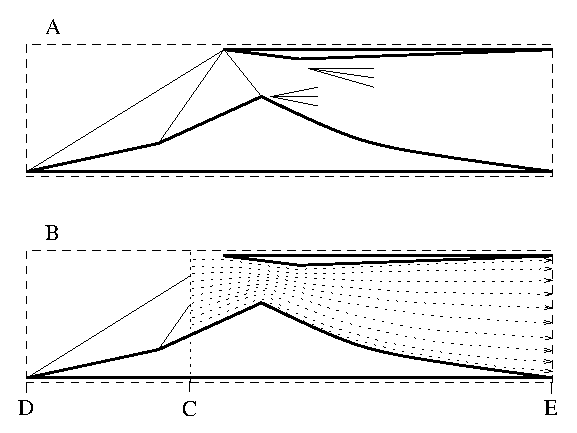
\includegraphics[width=5.0in]{engine.eps}
   \end{center}
\caption{Hypersonic engine schematic, along with the control volume 
         boundaries used to determine the thrust of the engine (top); 
         control volume boundaries around the engine along with the
         $x$-station under consideration ($x_2$) for the thrust potential (bottom);
         note that the flow is expanded from 
         station $x_2$ to station $x_3$ along an isentropic path.}
\label{fig:engine}
\end{figure}
%


Probably the most accurate manner in which to assess the losses part of
a flight vehicle is through the thrust potential method, as outlined in
Riggins {\it et al.}\cite{jpp:1997:riggins}. The idea is to integrate the
momentum flux expanded to a certain state (either ambiant pressure or exit
area) from the properties at a given streamwise cross-section, and to subtract
the integral of the momentum flux at the engine entrance:
%
\begin{equation}
 {\rm thrust~potential} = \int_{x=x_3} \left(\rho u^2 + P \right) \ordi A
   - \int_{x=x_1} \left(\rho u^2 + P \right) \ordi A
\end{equation}
%
For the engine configuration shown in  Fig.~\ref{fig:engine}, the thrust 
can be readily determined
through a control volume analysis as the difference between the outlet
momentum and the inlet momentum, minus the shear stresses on the top and bottom
boundaries of the engine. It is noted that the additive drag on the 
exterior of the engine is independant of the flowfield characteristics
of the engine, and is hence ignored for the determination of the thrust
potential. Further, Fig.~\ref{fig:engine} implies that the flow area at
the outlet matches the one at the inlet. This is not such a bad assumption
since scramjet flows are typically underexpanded\cite{book:1994:pratt}
with a pressure at the exit greater than ambiant, and the area cannot
be made much larger than the inlet area to minimize the drag forces on
the external surfaces.  We therefore decide to base our definition of 
the thrust potential on a fixed outlet area, equal to the inlet area. 
We further specify the pressure to be equal for all streamlines at the outlet,
but do not force a specific value. 

We will now express the thrust potential in concrete terms.
The turbulence kinetic energy along a streamline can be taken as
a constant if the source terms are neglected:
%
\begin{equation}
  k=k_2={\rm constant}
\end{equation}
%
From the momentum equation along a streamline (Euler formulation
with turbulence):
%
\begin{equation}
  \ordi P^\star = - \rho u \ordi u
  \label{eqn:thrust:momentum}
\end{equation}
%
and, at each point along the integration, the total enthalpy is identical
to the one at station $x_2$
%
\begin{equation}
  h + \frac{u^2}{2} =  h_2 + \frac{u_2^2}{2}
\end{equation}
%
Now, first guess an effective pressure at the outlet, $P_3^\star$. 
Integrate for each streamline
Eq.~(\ref{eqn:thrust:momentum}) from $P_2$ to $P_3$ and obtain consequently
$\rho_3$ and $u_3$. This can be done analytically in the case of a perfect
gas but numerically for a real gas. From the conservation of mass,
the expanded area $\ordi A_3$ of a flow particle occupying the
area $\ordi A_2$ then corresponds to:
%
\begin{equation}
  \ordi A_3  = \frac{\rho_2 u_2}{\rho_3 u_3} \ordi A_2
\end{equation}
%
with the area at $x=x_3$ equal to:
%
\begin{equation}
  A_3= \int \ordi A_3
\end{equation}
%
Since $A_3$ is desired to be equal to $A_1$, a Newton-Raphson iteration
can be performed to find a better guess to $P_3^\star$.





\subsection{Perfect Gas with Turbulence}

Recall that for a perfect gas with turbulence, we can say that:
%
\begin{equation}
\frac{\gamma}{\gamma-1} \ln \left( \frac{2 h_2+u_2^2-u_3^2+\frac{4}{3}k_2 \frac{\Cp}{R}}
                                 {2 h_2+\frac{4}{3}k_2 \frac{\Cp}{R}} \right)
  =  \ln \left(\frac{P_3^\star}{P_2^\star}\right)
\label{eqn:perfectv}
\end{equation}
%
or,
%
\begin{equation}
   \mfd u_3
  = \left[ 2 h_2+\frac{4}{3}k_2 \frac{\Cp}{R}+u_2^2
   -\left( 2 h_2 +\frac{4}{3}k_2 \frac{\Cp}{R} \right)
      \left(\frac{P_3^\star}{P_2^\star}\right)^\frac{\gamma-1}{\gamma}
    \right]^\frac{1}{2}
  \tag{\ref{eqn:perfectv}a}
  \label{eqn:perfectv-2}
\end{equation}
%
but, using the relationship $h+\frac{2}{3}k\frac{\Cp}{R}=a^2/(\gamma-1)$,
%
\begin{equation}
 \frameeqn{
   \mfd u_3
  = \left[ \frac{2 a_2^2}{\gamma-1}+u_2^2
   -\left( \frac{2 a_2^2}{\gamma-1} \right)
      \left(\frac{P_3^\star}{P_2^\star}\right)^\frac{\gamma-1}{\gamma}
    \right]^\frac{1}{2}
 }
  \tag{\ref{eqn:perfectv}b}
  \label{eqn:perfectv-final}
\end{equation}
%
And through the energy equation and the equation of state,
%
\begin{equation}
   h_2+u_2^2/2-u_3^2/2 +\frac{2}{3}\frac{\Cp}{R} k_2
 = \frac{\gamma}{\gamma-1} \frac{P_3^\star}{\rho_3}
  \label{eqn:perfectrho}
\end{equation}
%
or,
%
\begin{equation}
   \left( 2 h_2 +\frac{4}{3}\frac{\Cp}{R} k_2 \right) 
   \left( \frac{P_3^\star}{P_2^\star}\right)^{\frac{\gamma-1}{\gamma}}
 = \frac{2 \gamma}{\gamma-1} \frac{P_3^\star}{\rho_3}
  \tag{\ref{eqn:perfectrho}a}
\end{equation}
%
or,
%
\begin{equation}
   \left(  \frac{P^\star_2}{\rho_2} \right)
   \left( \frac{P_3^\star}{P_2^\star}\right)^{\frac{\gamma-1}{\gamma}}
 =  \frac{P_3^\star}{\rho_3}
  \tag{\ref{eqn:perfectrho}b}
\end{equation}
%
and,
%
\begin{equation}
 \frameeqn{\rho_3 = \rho_2 \left( \mfd \frac{P_3^\star}{P_2^\star} \right)^\frac{1}{\gamma}}
  \tag{\ref{eqn:perfectrho}c}
  \label{eqn:perfectrho-final}
\end{equation}
%
Through conservation of mass,
%
\begin{equation}
  \int \frac{\rho_2 u_2^\perp}{\rho_3 u_3} \ordi A_2 = A_3
  \label{eqn:perfectP3}
\end{equation}
%
where $u_2^\perp$ is the velocity component perpendicular to $\ordi A_2$.
At station $3$, the flow is assumed to be expanded with the streamlines
perpendicular to exit area, and the total velocity will correspond to
the velocity perpendicular to surface $A_3$.
Substituting expressions for $\rho_3$ and $u_3$ in the latter,
%
\begin{equation}
  \int \left. {\rho_2 u_2^\perp} \left/ \rho_2 \left( \mfd \frac{P_3^\star}{P_2^\star} \right)^\frac{1}{\gamma} 
  \left[ 2 h_2+\frac{4}{3}k_2 \frac{\Cp}{R}+u_2^2
   -\left( 2 h_2 +\frac{4}{3}k_2 \frac{\Cp}{R} \right)
      \left(\frac{P_3^\star}{P_2^\star}\right)^\frac{\gamma-1}{\gamma}
  \right]^\frac{1}{2}            
   \right. \ordi A_2 \right.= A_3
  \tag{\ref{eqn:perfectP3}a}
\end{equation} 
%
which can be recast to, using the sound speed $a^2=\frac{2}{3}\gamma k +(\gamma-1) h$:
%
\begin{equation}
  A_3=\mfd \int \left. {\rm M}_2^\perp  \left( \mfd \frac{P_2^\star}{P_3^\star} \right)^\frac{1}{\gamma}
  \left[ \frac{2}{\gamma-1}+{\rm M}_2^2
   - \frac{2}{\gamma-1}
      \left(\frac{P_3^\star}{P_2^\star}\right)^\frac{\gamma-1}{\gamma}
  \right]^{-\frac{1}{2}}
   \right. \ordi A_2
  \tag{\ref{eqn:perfectP3}b}
  \label{eqn:perfectP3-2}
\end{equation}
%
%
\begin{equation}
 \frameeqn{
  A_3=\mfd\int u_2^\perp   {P_2^\star}^\frac{1}{\gamma}
  \left/
  u_3 {P_3^\star}^\frac{1}{\gamma}
  \ordi A_2
   \right.
  }
  \tag{\ref{eqn:perfectP3}c}
  \label{eqn:perfectP3-final}
\end{equation}
%
from which $P_3^\star$ and $A_3$ are the only unknowns. For $P_3^\star$ user-specified,
$A_3$ can be readily determined. For $A_3$ user-specified, a Newton-Raphson
iteration can be used to find $P_3^\star$. Once $P_3^\star$ is determined from
Eq.~(\ref{eqn:perfectP3-final}), the thrust potential
can be directly integrated at the $x$-station of interest as
%
\begin{equation}
 {\rm thrust~potential} = \mfd\int \left(\rho_3 u_3^2 + P_3^\star \right)
     \frac{\rho_2 u_2^\perp}{\rho_3 u_3} \ordi A_2
   - \mfd\int \left(\rho_1 u_1^2 + P_1^\star \right) \ordi A_1
\end{equation}
%
where $\rho_3$  is substituted from  Eq.~(\ref{eqn:perfectrho-final}):
%
\begin{equation}
 \frameeqn{
  {\rm thrust~potential}=  \mfd\int \!\rho_2 u_{3} u_2^\perp
 + u_2^\perp {P^\star_2}^{\frac{1}{\gamma}}  \left/ u_{3}{P_3^\star}^{\frac{1-\gamma}{\gamma}}
    \right.\ordi A_2
   - \mfd\int \!\left(\rho u_1^2 + P_1^\star \right) \ordi A_1
 }
\end{equation}
%
where $u_3$  is taken from Eqs.~(\ref{eqn:perfectv-final}), and
$P_3^\star$ is found from Eq.~(\ref{eqn:perfectP3-final}) by user-specifying $A_3$.













\subsection{High-Temperature Gas with Turbulence}

The turbulent kinetic energy can be shown to be constant along a streamline
for the source terms neglected:
%
\begin{equation}
  k=k_2={\rm constant}
\end{equation}
%
From the momentum equation along a streamline (Euler formulation
with turbulence):
%
\begin{equation}
  \ordi P^\star = - \rho u \ordi u
\end{equation}
%
and, at each point along the integration, the total enthalpy is identical
to the one at station $x_2$
%
\begin{equation}
  h + \frac{u^2}{2} =  h_2 + \frac{u_2^2}{2}
\end{equation}
%
which basically gives a relationship between the temperature and the flow speed.
The last three equations can be combined with the equation of
state to form the following:
%
\begin{equation}
 \frameeqn{
  \mfd\frac{\ordi u}{\ordi P^\star} = - \frac{RT + \frac{2}{3}k_2}{P^\star u}
 }
  \label{eqn:thrust:momentum:final}
\end{equation}
%
If numerically integrated from point 2 to 3, 
the latter can give $u_3$ for $u_2$, $P^\star_2$ and $P^\star_3$ specified.
Now, first guess an effective pressure at the outlet, $P_3^\star$.
Integrate for each streamline
Eq.~(\ref{eqn:thrust:momentum:final}) from $P_2^\star$ to $P_3^\star$ and obtain consequently
$\rho_3$ and $u_3$.  Then, from conservation of mass principles,
the expanded area $\ordi A_3$ of a flow particle occupying the
area $\ordi A_2$ corresponds to:
%
\begin{equation}
   \ordi A_3  = \frac{\rho_2 u_2^\perp}{\rho_3 u_3} \ordi A_2
\end{equation}
%
where the superscript $\perp$ refers to taking the velocity component
perpendicular to the area $\ordi A_2$. 
The total area of the flow at $x=x_3$ equal to:
%
\begin{equation}
  \frameeqn{
    \mfd A_3= \int \frac{\rho_2 u_2^\perp}{\rho_3 u_3} \ordi A_2
  }
\end{equation}
%
Since $A_3$ is desired to be equal to $A_1$, a Newton-Raphson iteration
can be performed to find a better guess to $P_3^\star$. Finally, once
$P_3^\star$ is determined, the thrust potential can be expressed as:
%
\begin{equation}
 {\rm thrust~potential} = \mfd\int \left(\rho_3 u_3^2 + P_3^\star \right)
     \frac{\rho_2 u_2^\perp}{\rho_3 u_3} \ordi A_2
   - \mfd\int \left(\rho_1 u_1^2 + P_1^\star \right) \ordi A_1
\end{equation}
%
or
%
\begin{equation}
 \frameeqn{
 {\rm thrust~potential} = \mfd\int \frac{\rho_3 u_3^2 + P_3^\star}{\rho_3 u_3}  \ordi \dot{m}
   - \mfd\int \left(\rho_1 u_1^2 + P_1^\star \right) \ordi A_1
 }
\end{equation}
%









\subsection{Perfect Gas with Turbulence, Revisited}

The relationship for the stagnation pressure was proven previously to be:
%
\begin{equation}
  \mfd P^\circ
  =
   P^\star \left[ 1+ \frac{\gamma-1}{2} {\rm M}^2 \right]
   ^\frac{\gamma}{\gamma-1}
\end{equation}
%
The thrust potential is recalled to correspond to:
%
\begin{equation}
 \frameeqn{
  {\rm thrust~potential}=  \mfd\int_2 \! u_{3}
 + {P^\star}^{\frac{1}{\gamma}}  \left/ \rho u_{3}{P_3^\star}^{\frac{1-\gamma}{\gamma}}
    \right.\ordi \mdot
   - \mfd\int_1 \!\left(\rho u^2 + P^\star \right) \ordi A
 }
\end{equation}
%
while an expression for $u_3$ was shown previously to correspond to:
%
\begin{equation}
   \mfd u_3
  = a \left[ \frac{2 }{\gamma-1}+{\rm M}^2
   -\left( \frac{2 }{\gamma-1} \right)
      \left(\frac{P_3^\star}{P^\star}\right)^\frac{\gamma-1}{\gamma}
    \right]^\frac{1}{2}
\end{equation}
%
%
\begin{equation}
   \mfd u_3
  = a \sqrt{\frac{2 }{\gamma-1}} \left[ 1+\frac{\gamma-1}{2}{\rm M}^2
       -\left(\frac{P_3^\star}{P^\star}\right)^\frac{\gamma-1}{\gamma}
    \right]^\frac{1}{2}
\end{equation}
%
%
\begin{equation}
   \mfd u_3
  = a \sqrt{\frac{2 }{\gamma-1}} \left[ \left(\frac{P^\circ}{P^\star} \right)^\frac{\gamma-1}{\gamma}
       -\left(\frac{P_3^\star}{P^\star}\right)^\frac{\gamma-1}{\gamma}
    \right]^\frac{1}{2}
\end{equation}
%
say $j=(\gamma-1)/\gamma$, then,
%
\begin{equation}
  \frameeqn{
   \mfd u_3
  = a \sqrt{\frac{2 }{\gamma-1}} \left[ \frac{{P^\circ}^j-{P_3^\star}^j}{{P^\star}^j}
    \right]^\frac{1}{2}
  }
\end{equation}
%
Further, let's seek an expression for $\rho a^2$ knowing
$a^2=\frac{2}{3}\gamma k+(\gamma-1) h=\frac{2}{3}\gamma k+\gamma R T$:
%
\begin{equation}
  \rho a^2 = \frac{P^\star (\frac{2}{3}\gamma k+\gamma R T)}{R T +\frac{2}{3} k}
           = \gamma P^\star
\end{equation}
%
then, an expression for $\rho u_3$ would look like:
%
\begin{equation}
   \mfd \rho u_3
  = \frac{\gamma P^\star}{a} \sqrt{\frac{2 }{\gamma-1}} \left[ \frac{{P^\circ}^j-{P_3^\star}^j}{{P^\star}^j}
    \right]^\frac{1}{2}
\end{equation}
%
%
\begin{equation}
 \frameeqn{
   \mfd \rho u_3
  = \frac{\gamma}{a} \sqrt{\frac{2 }{\gamma-1}}
    \left[ {P^\circ}^j-{P_3^\star}^j \right]^\frac{1}{2}
    {P^\star}^\frac{\gamma+1}{2\gamma}
 }
\end{equation}
%
Now, we will seek to simplify the first integral of
the thrust potential equation using the obtained expressions
for $u_3$ and $\rho u_3$:
%
\begin{equation}
\begin{array}{l}
\mfd\int_2 \! u_{3}
 + {P^\star}^{\frac{1}{\gamma}}  \left/ \rho u_{3}{P_3^\star}^{\frac{1-\gamma}{\gamma}}
    \right.\ordi \mdot \alb
~~~~=\mfd\int_2 \! a \sqrt{\frac{2 }{\gamma-1}} \left[ \frac{{P^\circ}^j-{P_3^\star}^j}{{P^\star}^j}
    \right]^\frac{1}{2}
 + {P_3^\star}^{\frac{\gamma-1}{\gamma}} {P^\star}^{\frac{1}{\gamma}}  \left/
\frac{\gamma}{a} \sqrt{\frac{2 }{\gamma-1}}
    \left[ {P^\circ}^j-{P_3^\star}^j \right]^\frac{1}{2}
    {P^\star}^\frac{\gamma+1}{2\gamma}
    \right.\ordi \mdot \alb
~~~~=\mfd\int_2 \! a {P^\star}^{\frac{-j}{2}} \sqrt{\frac{2 }{\gamma-1}} \left[{P^\circ}^j-{P_3^\star}^j\right]^\frac{1}{2}
 + a {P_3^\star}^{\frac{\gamma-1}{\gamma}} {P^\star}^{\frac{1-\gamma}{2\gamma}}  \left/
   \sqrt{\frac{2 \gamma^2}{\gamma-1}}
    \left[ {P^\circ}^j-{P_3^\star}^j \right]^\frac{1}{2}
    \right.\ordi \mdot \alb
~~~~=\mfd\int_2 \!
  \frac{
   a {P^\star}^{\frac{-j}{2}}
  }{
   \sqrt{\frac{2 \gamma^2}{\gamma-1}}
    \left[ {P^\circ}^j-{P_3^\star}^j \right]^\frac{1}{2}
  }
  \left[
    \frac{2 \gamma}{\gamma-1} \left[{P^\circ}^j-{P_3^\star}^j\right]
 + {P_3^\star}^j
  \right] \ordi \mdot\alb
~~~~=\mfd\int_2 \!
  \frac{
   a {P^\star}^{\frac{-j}{2}}
  }{
   \sqrt{2 j \gamma}
    \left[ {P^\circ}^j-{P_3^\star}^j \right]^\frac{1}{2}
  }
  \left[ 2 {P^\circ}^j + (j-2) {P_3^\star}^j \right] \ordi \mdot\alb
~~~~=\mfd\int_2 \!
  \frac{
   a \left[ 2 {P^\circ}^j + (j-2) {P_3^\star}^j \right]
  }{
    \left[2 j \gamma {P^\star}^j ( {P^\circ}^j-{P_3^\star}^j) \right]^\frac{1}{2}
  }
   \ordi \mdot\alb
\end{array}
\end{equation}
%
therefore,
%
\begin{equation}
\frameeqn{
\mfd\int_2 \! u_{3}
 + {P^\star}^{\frac{1}{\gamma}}  \left/ \rho u_{3}{P_3^\star}^{\frac{1-\gamma}{\gamma}}
    \right.\ordi \mdot
   =\mfd\int_2 \!
  \frac{
   a \left[ 2 {P^\circ}^j + (j-2) {P_3^\star}^j \right]
  }{
    \left[2 j \gamma {P^\star}^j ( {P^\circ}^j-{P_3^\star}^j) \right]^\frac{1}{2}
  }
   \ordi \mdot
 }
\end{equation}
%


\subsubsection{Special Case for Vanishing Back Pressure}

Let's assume that $P_3^\star=0$. Then,
%
%
\begin{equation}
\begin{array}{l}
\mfd\int_2 \! u_{3}
 + {P^\star}^{\frac{1}{\gamma}}  \left/ \rho u_{3}{P_3^\star}^{\frac{1-\gamma}{\gamma}}
    \right.\ordi \mdot \alb
~~~~=\mfd\int_2 \!
  \frac{
   a \left[ 2 {P^\circ}^j + (j-2) {P_3^\star}^j \right]
  }{
    \left[2 j \gamma {P^\star}^j ( {P^\circ}^j-{P_3^\star}^j) \right]^\frac{1}{2}
  }
   \ordi \mdot
=\mfd\int_2 \!
  \frac{
   a \left[ 2 {P^\circ}^j \right]
  }{
    \left[2 j \gamma {P^\star}^j {P^\circ}^j\right]^\frac{1}{2}
  }
   \ordi \mdot
=\mfd\int_2 \!
  \left[
  \frac{
   2 a^2  {P^\circ}^j
  }{
     j \gamma {P^\star}^j
  }
  \right]^{1/2}
   \ordi \mdot
\end{array}
\end{equation}
%
and, from the relationship between the stagnation pressure ratio and the stagnation
temperature ratio:
%
%
\begin{align*}
\int_2& \! u_{3}
 + {P^\star}^{\frac{1}{\gamma}}  \left/ \rho u_{3}{P_3^\star}^{\frac{1-\gamma}{\gamma}}
    \right.\ordi \mdot \alb
&=\!\mfd\int_2 \!
  \left[
  \frac{2 (\gamma R T + \frac{2}{3} \gamma k)}{j \gamma}
  \left( \frac{T^\circ}{T} - \frac{\gamma^2-\gamma}{6} {\rm M}^2 {\rm M}^2\turb \right)
  \right]^{1/2}
   \ordi \mdot\alb
&=\!\mfd \int_2 \!
  \frac{1}{\sqrt{j}} \left[
  \left( 2 R T + \frac{4}{3} k \right)
  \left( \frac{T^\circ}{T} - \frac{\gamma^2-\gamma}{6} {\rm M}^2 {\rm M}^2\turb \right)
  \right]^{1/2}
   \ordi \mdot\alb
&=\!\mfd \int_2 \!
  \frac{1}{\sqrt{j}}\left[
  2 R T^\circ -  2 R T \frac{\gamma^2-\gamma}{6} {\rm M}^2 {\rm M}^2\turb
  + \frac{4}{3} k \frac{T^\circ}{T} -  \frac{4}{3} k \frac{\gamma^2-\gamma}{6} {\rm M}^2 {\rm M}^2\turb
  \right]^{1/2}
   \ordi \mdot\alb
&=\!\mfd \int_2 \!
  \frac{1}{\sqrt{j}}\left[
  2 R T^\circ +  \frac{4}{3} k \left( -\frac{\gamma-1}{2} {\rm M}^2
  + \frac{T^\circ}{T} -  \frac{\gamma^2-\gamma}{6} {\rm M}^2 {\rm M}^2\turb \right)
  \right]^{1/2}
   \ordi \mdot\alb
&=\!\mfd \int_2 \!
  \frac{1}{\sqrt{j}}\left[
  2 R T^\circ +  \frac{4}{3} k \left( -\frac{\gamma-1}{2} {\rm M}^2
  +1+\mfd\frac{\gamma-1}{2} {\rm M}^2
                     \left(1+\mfd\frac{\gamma}{3} {\rm M}\turb^2 \right)  -  \frac{\gamma^2-\gamma}{6} {\rm M}^2 {\rm M}^2\turb \right)
  \right]^{1/2}
  \!\!\!\!\! \ordi \mdot\alb
\end{align*}
%
and finally,
%
\begin{equation}
\frameeqn{
\mfd\int_2 \! u_{3}
 + {P^\star}^{\frac{1}{\gamma}}  \left/ \rho u_{3}{P_3^\star}^{\frac{1-\gamma}{\gamma}}
    \right.\ordi \mdot
   =\int_2 \!
  \left[
    \frac{2\gamma}{\gamma-1} \left( R T^\circ +  \frac{2}{3} k \right)
  \right]^\frac{1}{2}
   \ordi \mdot
 }
\end{equation}
%
which shows clearly that the thrust potential is \emph{only} a function of
the stagnation temperature and the turbulence kinetic energy, and \emph{not}
of the stagnation pressure, in the particular case of vanishing pressure
at the exit.


\subsubsection{Expressing the Thrust Potential as a Function of the Stagnation
               Temperature}

Starting from where we left off,
%
\begin{align*}
\mfd\int_2& \! u_{3}
 + {P^\star}^{\frac{1}{\gamma}}  \left/ \rho u_{3}{P_3^\star}^{\frac{1-\gamma}{\gamma}}
    \right.\ordi \mdot\alb
   &=\mfd\int_2 \!
  \frac{
   a \left[ 2 {P^\circ}^j + (j-2) {P_3^\star}^j \right]
  }{
    \left[2 j \gamma {P^\star}^j ( {P^\circ}^j-{P_3^\star}^j) \right]^\frac{1}{2}
  }
   \ordi \mdot\alb
   &=\mfd\int_2 \!
    \left[ 2+ (j-2) \frac{{P_3^\star}^j}{{P^\circ}^j} \right]
  \left/
    \left[\frac{2\gamma j}{a^2} \frac{{P^\star}^j}{{P^\circ}^j} \left( 1-\frac{{P_3^\star}^j}{{P^\circ}^j}\right) \right]^\frac{1}{2}
  \right.
   \ordi \mdot\alb
   &=\mfd\int_2 \!
    \left[ 2+ (j-2) \frac{{P_3^\star}^j}{{P^\circ}^j} \right]
  \left/
    \left[\frac{2 j}{R T^\circ + \frac{2}{3} k} \left( 1-\frac{{P_3^\star}^j}{{P^\circ}^j}\right) \right]^\frac{1}{2}
  \right.
   \ordi \mdot\alb
  &=\mfd\int_2 \!
    \left(\frac{2 R T^\circ + \frac{4}{3} k}{j}\right)^\frac{1}{2}
    \left[ 1+ \left(\frac{j}{2}-1\right) \frac{{P_3^\star}^j}{{P^\circ}^j} \right]
  \left/
    \left( 1-\frac{{P_3^\star}^j}{{P^\circ}^j}\right)^\frac{1}{2}
  \right.
   \ordi \mdot
\end{align*}
%
%
\begin{figure}[ht]
 \begin{center}
   \psfrag{X}[t][t][1][0]{$P^\circ/P_3^\star$}
   \psfrag{Y}[b][b][1][0]{$\left[ 1+ \left(\frac{j}{2}-1\right) \frac{{P_3^\star}^j}{{P^\circ}^j} \right]
  \left/
    \left( 1-\frac{{P_3^\star}^j}{{P^\circ}^j}\right)^\frac{1}{2}
  \right.$}
   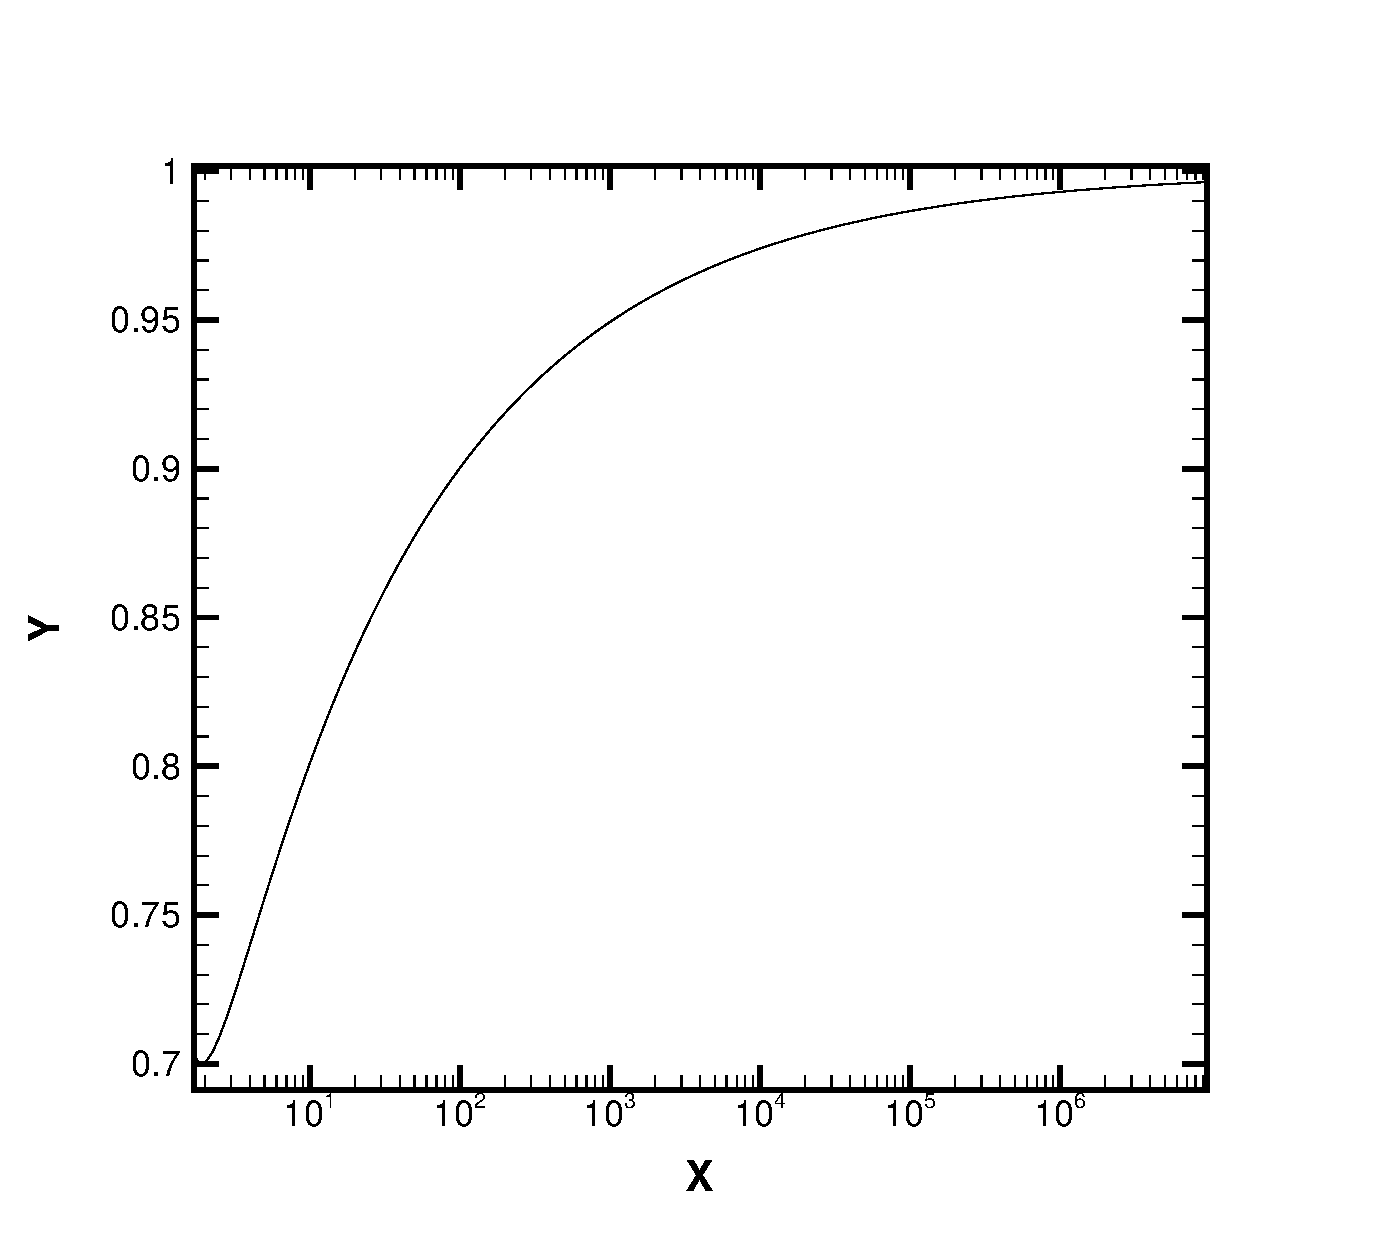
\includegraphics[width=3.3in]{pstag_over_p3.eps}
   \caption{Non-dimensional part of the thrust potential involving the
            stagnation pressure $P^\circ$ and back pressure, for
            $\gamma=1.4$; it is reminded that $j=(\gamma-1)/\gamma$.}
 \end{center}
\end{figure}
%
%
\begin{figure}[ht]
 \begin{center}
   \psfrag{X}[t][t][1][0]{$RT^\circ$}
   \psfrag{Y}[b][b][1][0]{$\left(\frac{2 R T^\circ}{j}\right)^\frac{1}{2}$ [Ns/kg]}
   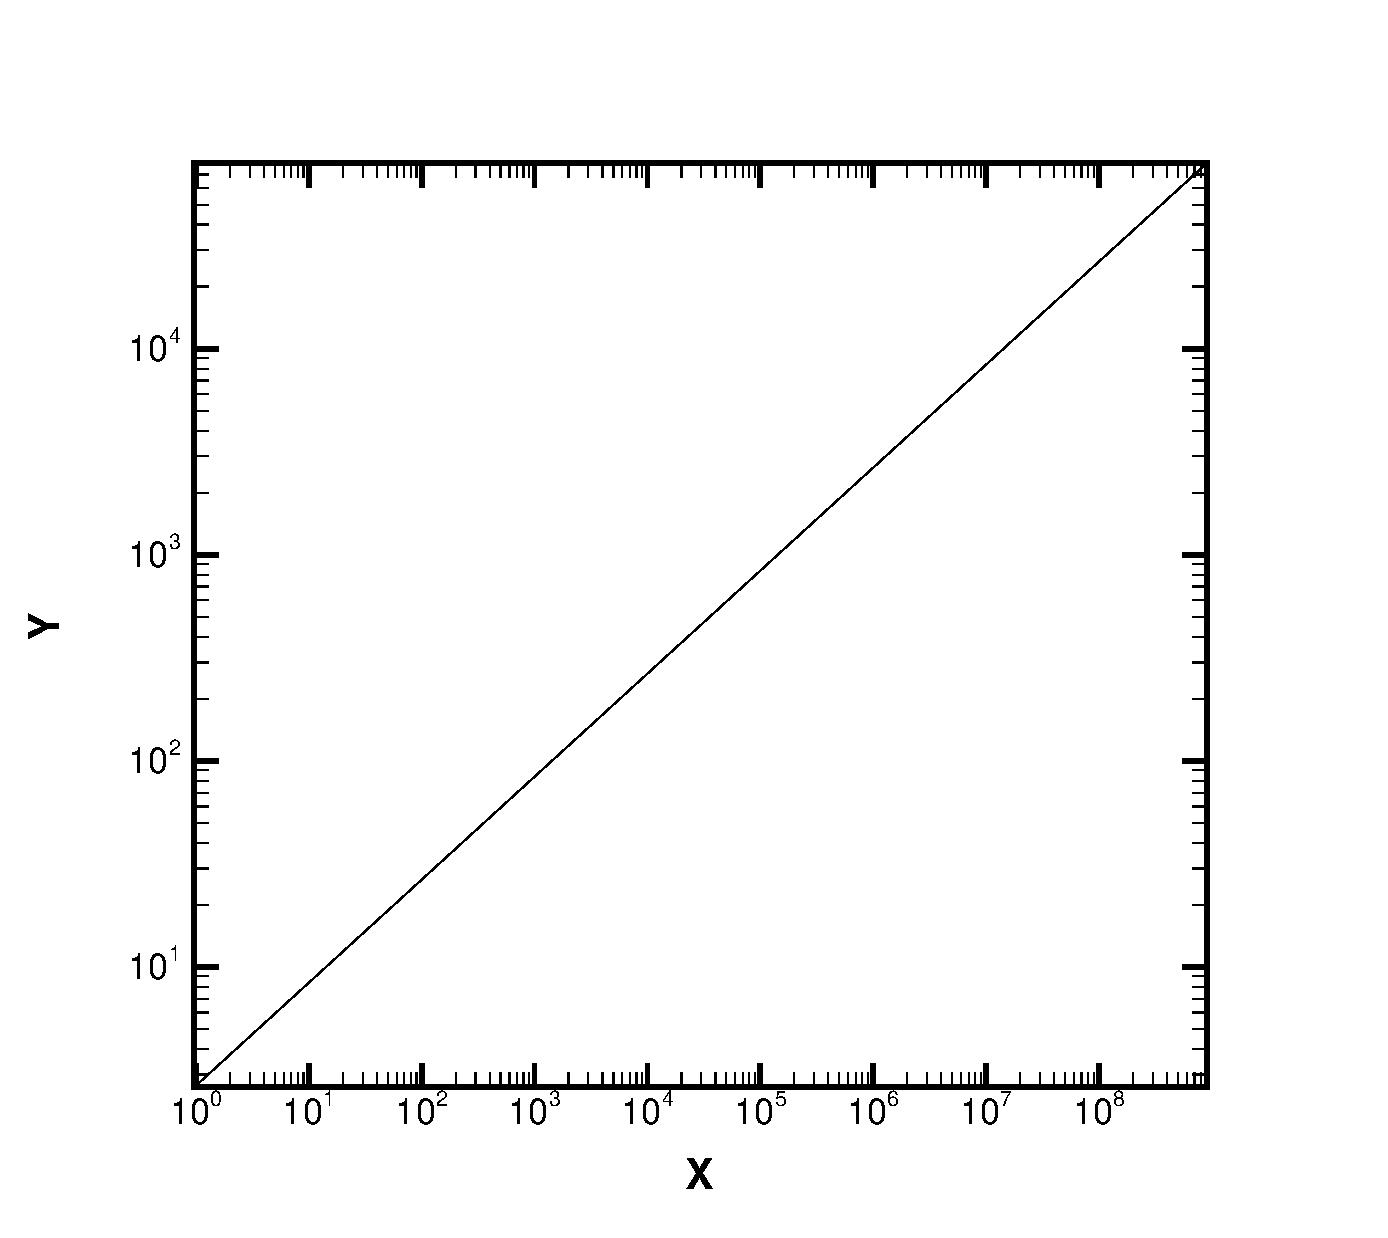
\includegraphics[width=3.3in]{RTstag.eps}
   \caption{Part of the thrust potential involving the
            stagnation temperature $T^\circ$ neglecting turbulence ($k=0$) with
            $\gamma=1.4$; it is reminded that $j=(\gamma-1)/\gamma$.}
 \end{center}
\end{figure}
%

  \bibliographystyle{warpdoc}
  \bibliography{all}


\end{document}






